\documentclass[sigconf,nonacm]{acmart}

\setcopyright{none}
\settopmatter{printacmref=false}
\renewcommand\footnotetextcopyrightpermission[1]{}
\pagestyle{plain}

\usepackage{booktabs}
\usepackage{tabularx}
\usepackage{multirow}
\usepackage{amsmath}
\let\Bbbk\relax
\usepackage{amssymb}
\usepackage{tikz}
\usepackage{pgfplots}
\pgfplotsset{compat=1.18}
\usepackage{listings}
\usepackage{url}
\urlstyle{rm}

\usetikzlibrary{arrows.meta,positioning,calc,shapes.geometric,
                decorations.pathreplacing,patterns}

%% ── colour palette ───────────────────────────────────────────────────────────
\definecolor{cblu} {RGB}{ 50,110,190}
\definecolor{cgrn} {RGB}{ 40,150, 70}
\definecolor{cora} {RGB}{210,110, 30}
\definecolor{cred} {RGB}{200, 50, 50}
\definecolor{cyel} {RGB}{190,165,  0}
\definecolor{cpur} {RGB}{130, 50,170}
\definecolor{cgry} {RGB}{100,100,100}

%% ── code listing style ───────────────────────────────────────────────────────
\lstset{
  basicstyle=\ttfamily\fontsize{7.5pt}{9pt}\selectfont,
  keywordstyle=\bfseries\color{cblu!80},
  commentstyle=\itshape\color{cgry!65},
  stringstyle=\color{cred!70},
  language=C++,
  breaklines=true,
  frame=single,
  framesep=3pt,
  xleftmargin=4pt,
  xrightmargin=4pt,
  numberstyle=\tiny\color{cgry!60},
  numbers=left,
  numbersep=4pt,
  showstringspaces=false,
  morekeywords={uint64\_t,int64\_t}
}

\begin{CCSXML}
<ccs2012>
  <concept>
    <concept_id>10002978.10003006.10003007</concept_id>
    <concept_desc>Security and privacy~Cryptography</concept_desc>
    <concept_significance>500</concept_significance>
  </concept>
  <concept>
    <concept_id>10002978.10003006.10003008</concept_id>
    <concept_desc>Security and privacy~Side-channel analysis and countermeasures</concept_desc>
    <concept_significance>500</concept_significance>
  </concept>
  <concept>
    <concept_id>10002978.10003006.10003007.10003009</concept_id>
    <concept_desc>Security and privacy~Homomorphic encryption</concept_desc>
    <concept_significance>300</concept_significance>
  </concept>
</ccs2012>
\end{CCSXML}

\ccsdesc[500]{Security and privacy~Cryptography}
\ccsdesc[500]{Security and privacy~Side-channel analysis and countermeasures}
\ccsdesc[300]{Security and privacy~Homomorphic encryption}

\title{RevEAL: Methodology, Security Implications, and Defenses for the First Single-Trace Side-Channel Attack on a Homomorphic Encryption Library}

\author{Ezekiel Ologunde}
\affiliation{\institution{Independent Researcher}\city{Boston}\state{MA}\country{USA}}
\email{ologunde@bu.edu}

\begin{abstract}
The RevEAL attack, introduced by Aydin et al.\ in 2022, represents the first
demonstrated side-channel attack capable of recovering plaintext from a single power
trace collected during encryption with the Microsoft SEAL homomorphic encryption
library. The attack exploits two classes of implementation vulnerability in the
Gaussian noise sampling routine used by SEAL's BFV scheme prior to version~3.6:
control-flow leakage arising from a conditional branch on the sign of each sampled
coefficient, and data-flow leakage from the Hamming-weight patterns of data written
to memory before and after a 2's-complement negation. This paper provides a
structured analysis of the RevEAL methodology, traces each leakage point through
the vulnerable source code, quantifies the resulting security degradation using the
DBDD lattice framework, and evaluates the recommended software-level countermeasures.
Our analysis confirms that sign-bit leakage alone reduces a nominal 128-bit-secure
parameter set to approximately $2^{84.3}$ security, while full exploitation of all
three leakage channels reduces effective security to approximately $2^{4.4}$---a
complete break. We show why conventional hardware masking is structurally
ineffective against single-trace attacks and argue that constant-time coding
practices and centered binomial distribution sampling are both necessary and
sufficient to close the vulnerability. The analysis generalises beyond SEAL to any
FHE implementation that samples noise through secret-dependent branching, and
provides a template for implementation-level security audits of homomorphic
encryption libraries.
\end{abstract}

\keywords{homomorphic encryption, side-channel attack, single-trace analysis,
Microsoft SEAL, Gaussian sampling, power analysis, constant-time coding, BFV scheme,
LWE, RLWE}

\begin{document}
\hfuzz=5pt
\maketitle

%%─────────────────────────────────────────────────────────────────────────────
\section{Introduction}
%%─────────────────────────────────────────────────────────────────────────────

Homomorphic encryption (HE) enables computation on encrypted data without
decryption---a capability with transformative implications for privacy-preserving
cloud computing, secure multi-party computation, and confidential machine learning
inference. The mathematical security of leading HE schemes such as the
Brakerski-Fan-Vercauteren (BFV) and Cheon-Kim-Kim-Song (CKKS) schemes is grounded
in the conjectured hardness of the Ring Learning With Errors (RLWE) problem, for
which no efficient classical or quantum algorithm is known~\cite{brakerski2012,fan2012}.

However, mathematical security proofs characterise the hardness of breaking the
scheme given only its inputs and outputs---they do not account for the physical
behaviour of the hardware that executes the cryptographic code. Side-channel attacks
exploit precisely this gap: by observing power consumption, electromagnetic emissions,
or timing, an adversary with physical access to the device can extract information
that the mathematical model treats as hidden. This threat is well-established for
classical symmetric and asymmetric cryptography~\cite{kocher1999,messerges2000}, but
until 2022 no side-channel attack had been demonstrated against a homomorphic
encryption library.

The RevEAL attack, published by Aydin et al.~\cite{aydin2022reveal}, closes this gap.
It is the first demonstrated side-channel attack on a production HE library that
recovers plaintext from a \emph{single} power trace. Its target is the Gaussian
noise sampling routine in Microsoft SEAL~\cite{sealcrypto} prior to version~3.6.
The attack exploits two specific implementation choices---a conditional branch on the
sign of each sampled coefficient, and subsequent data-dependent memory writes---to
recover the error polynomial used during encryption. Once the error polynomial is
known, a standard lattice reduction solver can decrypt the ciphertext with negligible
residual cost.

\subsection{Scope and Contributions}

This paper provides a structured academic analysis of RevEAL, addressing the
following questions:

\begin{enumerate}
  \item How do specific implementation choices in SEAL's Gaussian sampling routine
        create exploitable side-channel leakage, and what is the precise mechanism
        linking each code construct to a measurable physical signal?
  \item What is the quantitative impact of each leakage channel on the security level
        of SEAL-BFV, expressed in terms of BKZ block size and equivalent bit security?
  \item Why are conventional hardware countermeasures---in particular, masking---
        ineffective against RevEAL, and what properties of the attack render them
        structurally insufficient?
  \item What software-level defenses close the vulnerability, and what trade-offs do
        they entail?
\end{enumerate}

The contributions of this paper are: (1) a self-contained technical exposition of
the RevEAL attack chain from vulnerable code to lattice decryption; (2) a
consolidated quantitative security analysis with the underlying parameter set; (3) a
principled evaluation of countermeasure effectiveness grounded in the single-trace
threat model; and (4) generalised design guidance for implementation-level security
audits of HE libraries.

\subsection{Relationship to Prior Work}

Power analysis attacks were first formalised by Kocher et al.~\cite{kocher1999} for
RSA and DES, and subsequently extended to AES and elliptic curve implementations.
Template attacks~\cite{chari2002} introduced the idea of profiling a device to
build precise leakage models, enabling single-trace extraction of secrets from one
measurement. Horizontal side-channel analysis~\cite{walter2001} exploits the internal
structure of a single cryptographic operation (rather than averaging across many)
and is the analytical framework closest to RevEAL.

In the post-quantum setting, Ravi et al.~\cite{ravi2019} demonstrated side-channel
attacks on NTRU and lattice-based KEMs, and Pessl et al.~\cite{pessl2019} attacked
the noise sampling of New Hope. RevEAL extends this line of work to the FHE setting,
where the challenge is qualitatively different: each encryption uses independent fresh
randomness, precluding multi-trace differential power analysis (DPA) approaches that
rely on repeated encryptions of the same plaintext.

%%─────────────────────────────────────────────────────────────────────────────
\section{Background}
%%─────────────────────────────────────────────────────────────────────────────

\subsection{The BFV Homomorphic Encryption Scheme}

The BFV scheme~\cite{fan2012} operates in the polynomial ring
$R_q = \mathbb{Z}_q[X]/(X^n + 1)$, where $n$ is a power of two (the polynomial
degree, also called the ring dimension) and $q$ is the ciphertext modulus.
A BFV ciphertext encrypting a plaintext $\mathbf{m} \in R_t$
(where $t \ll q$ is the plaintext modulus) takes the form:
\[
  \mathbf{c} = (c_0,\ c_1) = \bigl([\mathbf{a} \cdot \mathbf{s} + \mathbf{e} + \Delta\mathbf{m}]_q,\
                                    [-\mathbf{a}]_q\bigr)
\]
where $\mathbf{a} \in R_q$ is a uniformly random polynomial, $\mathbf{s} \in R_q$
is the secret key, $\Delta = \lfloor q/t \rfloor$ is a scaling factor, and
$\mathbf{e} \in R_q$ is the \emph{noise} (error) polynomial. The security of the
scheme rests on the RLWE assumption: given $(\mathbf{a}, \mathbf{a}\cdot\mathbf{s} +
\mathbf{e})$, it is computationally infeasible to recover $\mathbf{s}$ (or
$\mathbf{e}$) without the secret key.

The noise polynomial $\mathbf{e}$ is sampled coefficient-by-coefficient from a
discrete Gaussian distribution $\chi_\sigma = D_{\mathbb{Z}, \sigma}$ with standard
deviation $\sigma$. The noise must be small (coefficients much less than $q$) so
that decryption---which essentially rounds off the noise---succeeds. The
\emph{choice of how to implement} this sampling in software is the root cause of
the RevEAL vulnerability.

\subsection{SEAL's Gaussian Sampling Implementation (Pre-v3.6)}

Microsoft SEAL~\cite{sealcrypto} implements BFV and CKKS. Prior to version~3.6,
the function \texttt{set\_poly\_coeffs\_normal} sampled each coefficient from the
discrete Gaussian and stored it in the output polynomial. The core loop, simplified
from the original C++ source, is shown in Listing~\ref{lst:vuln}.

\begin{lstlisting}[label=lst:vuln, caption={Vulnerable Gaussian sampling loop in SEAL pre-v3.6 (simplified from Aydin et al.).}]
for (size_t i = 0; i < n; i++) {
    int64_t noise = sample_gaussian(sigma); // secret
    if (noise < 0) {           // BRANCH on sign (*)
        noise = -noise;        // NEGATION of |noise| (**)
        poly[i] = noise;       // STORE |noise|
        poly[i] = -poly[i];    // RESTORE sign
    } else {
        poly[i] = noise;       // STORE positive value
    }
}
\end{lstlisting}

Three operations in this loop are marked as leakage sources:
\begin{itemize}
  \item Line~5 (\texttt{if (noise < 0)}): a branch whose outcome depends on the
        sign of the secret sample.
  \item Lines~6--7 (negation and store): data-dependent memory writes whose power
        consumption is proportional to the Hamming weight of the stored value.
  \item Lines~6 (negation): a 2's-complement operation whose input and output differ
        in Hamming weight in a value-dependent way.
\end{itemize}

These three constructs form the three attack channels exploited by RevEAL, which are
analysed in detail in Section~\ref{sec:attack}.

\subsection{Power-Based Side-Channel Models}

The RevEAL attack is built on two standard leakage models:

\textbf{Control-flow leakage.} When a processor takes a conditional branch, it
executes a different sequence of instructions than when it does not. Even at the
architectural level, the instruction count, pipeline state, and memory access
pattern differ between the two branches. These differences produce measurable
differences in power consumption. In the Hamming-weight model, the power consumed
executing a sequence of instructions is approximately proportional to the number of
bits that transition in the processor's registers and bus during that
sequence~\cite{mangard2007}.

\textbf{Data-flow leakage (Hamming weight).} When a value is written to memory or
processed through the ALU, the power consumed is approximately proportional to the
Hamming weight (number of set bits) of the value. An 8-bit value of $3 = 0000\,0011$
consumes less power than $255 = 1111\,1111$. This is the basis for simple power
analysis (SPA) and template attacks on stored values~\cite{mangard2007}.

\subsection{Template Attacks}

A template attack~\cite{chari2002} has two phases: a \emph{profiling} phase in which
the attacker characterises the device's leakage distribution for each secret value
class (building a ``template''), and an \emph{online} phase in which a single
observed trace is matched against templates to identify the most likely secret value.
Template attacks are optimal in an information-theoretic sense---they make maximum
use of the available leakage---and can succeed with a single trace if the templates
are built on sufficient profiling data. RevEAL uses template analysis throughout:
Aydin et al.\ profiled SEAL's sampling routine using 220{,}000 traces and then
performed the actual attack on a single fresh measurement~\cite{aydin2022reveal}.

%%─────────────────────────────────────────────────────────────────────────────
\section{The RevEAL Attack Methodology}
\label{sec:attack}
%%─────────────────────────────────────────────────────────────────────────────

RevEAL proceeds in four sequential steps, each exploiting one of the identified
leakage channels. Figure~\ref{fig:attack_flow} provides an overview.

\begin{figure}[h]
\centering
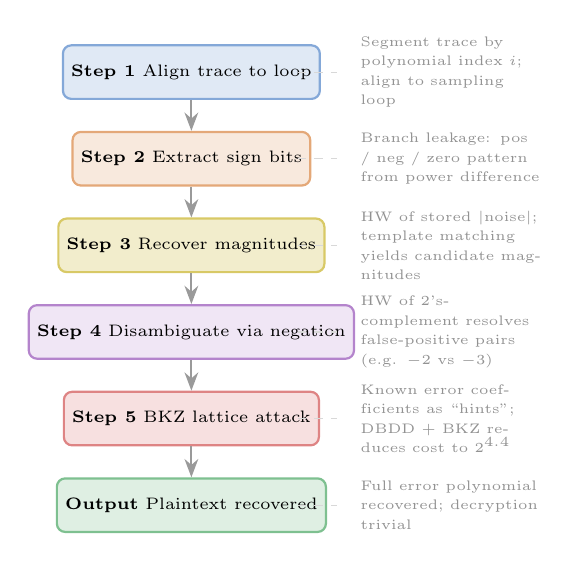
\begin{tikzpicture}[
  font=\fontsize{6.5pt}{8pt}\selectfont,
  >=Stealth,
  stg/.style={rectangle, rounded corners=3pt, draw, thick,
              minimum width=2.6cm, minimum height=0.68cm,
              text centered, inner sep=3pt},
  ann/.style={font=\fontsize{5.5pt}{7pt}\selectfont, text=cgry!70,
              align=left, text width=2.3cm},
  arr/.style={-{Stealth}, thick, cgry!65}
]
  \node[stg, fill=cblu!15, draw=cblu!60]   (s1) at (0, 0.00)
    {\textbf{Step 1} Align trace to loop};
  \node[stg, fill=cora!15, draw=cora!60]   (s2) at (0,-1.10)
    {\textbf{Step 2} Extract sign bits};
  \node[stg, fill=cyel!20, draw=cyel!60]   (s3) at (0,-2.20)
    {\textbf{Step 3} Recover magnitudes};
  \node[stg, fill=cpur!12, draw=cpur!60]   (s4) at (0,-3.30)
    {\textbf{Step 4} Disambiguate via negation};
  \node[stg, fill=cred!15, draw=cred!60]   (s5) at (0,-4.40)
    {\textbf{Step 5} BKZ lattice attack};
  \node[stg, fill=cgrn!15, draw=cgrn!60]   (s6) at (0,-5.50)
    {\textbf{Output} Plaintext recovered};

  \foreach \a/\b in {s1/s2,s2/s3,s3/s4,s4/s5,s5/s6}
    \draw[arr] (\a)--(\b);

  \node[ann] at (3.3, 0.00) {Segment trace by polynomial index $i$; align to sampling loop};
  \node[ann] at (3.3,-1.10) {Branch leakage: pos / neg / zero pattern from power difference};
  \node[ann] at (3.3,-2.20) {HW of stored $|$noise$|$; template matching yields candidate magnitudes};
  \node[ann] at (3.3,-3.30) {HW of 2's-complement resolves false-positive pairs (e.g. $-2$ vs $-3$)};
  \node[ann] at (3.3,-4.40) {Known error coefficients as ``hints''; DBDD + BKZ reduces cost to $2^{4.4}$};
  \node[ann] at (3.3,-5.50) {Full error polynomial recovered; decryption trivial};

  \foreach \y in {0.00,-1.10,-2.20,-3.30,-4.40,-5.50}
    \draw[dashed, cgry!25] (1.35,\y)--(1.85,\y);
\end{tikzpicture}
\caption{RevEAL attack flow from a single power trace to plaintext recovery. Steps~2,
  3, and~4 each correspond to one of the three leakage channels in the vulnerable
  Gaussian sampling code.}
\label{fig:attack_flow}
\end{figure}

\subsection{Step 1: Trace Alignment and Loop Segmentation}

The outer loop in the vulnerable code (Listing~\ref{lst:vuln}) iterates exactly $n$
times---once per polynomial coefficient. Because $n$ is a public parameter (typically
$n = 4096$ or $n = 8192$ for the 128-bit parameter sets), the attacker knows how
many iterations to expect and can segment the trace by index $i$. The trace is
aligned to the start of the sampling routine using standard trace-alignment techniques
(e.g., Sum of Absolute Differences on a known trigger signal). Once aligned, the
trace is partitioned into $n$ windows, one per coefficient, each of which will be
analysed independently. This step exploits no secret information---it merely
establishes the correspondence between trace segments and polynomial
indices~\cite{aydin2022reveal}.

\subsection{Step 2: Sign Bit Extraction via Control-Flow Leakage}

With the trace segmented, the attacker analyses the portion of each window
corresponding to the conditional branch at line~5 of Listing~\ref{lst:vuln}:
\texttt{if (noise < 0)}.

When \texttt{noise} is positive or zero, the processor takes the \texttt{else}
branch, executing only the assignment \texttt{poly[i] = noise}. When \texttt{noise}
is negative, the processor takes the \texttt{if} branch, which executes both the
negation (\texttt{noise = -noise}) and two stores. These two execution paths consume
demonstrably different power: the negative path executes more instructions (and a
nontrivial 2's-complement operation) than the positive path, producing a distinct
power signature~\cite{aydin2022reveal}.

The attacker uses template matching to classify each window into one of three
categories: positive, negative, or zero. Aydin et al.\ report \textbf{100\% success
rate} for this step~\cite{aydin2022reveal}---every coefficient's sign (or zero
status) is correctly recovered from a single trace. This result is consistent with
the theoretical expectation: the branch outcome changes the instruction stream
deterministically, creating a reliable physical distinction that template analysis
can exploit without any averaging across traces.

After this step, the attacker knows the exact sign pattern of the entire error
polynomial $\mathbf{e}$: which coefficients are positive, which are negative, and
which are zero.

\subsection{Step 3: Magnitude Recovery via Data-Flow Leakage}

Knowing the sign of each coefficient is valuable but not sufficient for a complete
attack. The attacker must also determine the magnitude $|e_i|$ of each coefficient.
This information is sought from the data-flow leakage of the assignment
\texttt{poly[i] = noise} (or \texttt{poly[i] = |noise|} in the negative branch).

When a value is written to memory, the power consumed by the bus and memory interface
is approximately proportional to the Hamming weight of the value. By comparing the
power trace at the store instruction against pre-built templates for small integers
(the coefficients are small by design---Gaussian noise with $\sigma \approx 3.2$ has
overwhelming probability of being in the range $[-16, 16]$), the attacker obtains a
candidate list of magnitudes for each coefficient. Formally, the attacker constructs
the set:
\[
  \mathcal{C}_i = \bigl\{ v \in \mathbb{Z}_{\geq 0}\ :\ \mathrm{HW}(v) = h_i \bigr\}
\]
where $h_i$ is the observed Hamming weight at index $i$. Because multiple distinct
small integers share the same Hamming weight (e.g., $2 = 0010$ and $4 = 0100$ both
have $\mathrm{HW} = 1$), the candidate set $\mathcal{C}_i$ typically contains more
than one element. This ambiguity is the ``false-positive'' problem noted in the
original paper~\cite{aydin2022reveal}.

\subsection{Step 4: Disambiguation via Negation Leakage}

The false-positive ambiguity from Step~3 is resolved by a third leakage channel:
the 2's-complement negation at line~6 of Listing~\ref{lst:vuln}, which executes
only for negative coefficients (identified in Step~2).

The key observation is that two integers sharing the same Hamming weight do
\emph{not} generally share the same Hamming weight after 2's-complement negation.
The 2's complement of $v$ is $\bar{v} + 1$ (bitwise complement plus one), which
redistributes the set bits. As the paper illustrates:
$-2 = 1111\ldots1110$ and $-3 = 1111\ldots1101$ have the same Hamming weight
in their stored (sign-extended) form, but when negated:
$2 = 0000\ldots0010$ has $\mathrm{HW} = 1$ while $3 = 0000\ldots0011$ has
$\mathrm{HW} = 2$~\cite{aydin2022reveal}. The power traces at the negation step
therefore differ, allowing the attacker to distinguish $-2$ from $-3$.

By observing the power consumption at the negation instruction for all
negative-signed coefficients (from Step~2), the attacker eliminates the false
positives from Step~3 and recovers the exact magnitude with high probability. The
combined result of Steps~2--4 is the recovery of the complete signed error
polynomial $\mathbf{e}$, with each coefficient's sign and magnitude determined from
a single trace.

Figure~\ref{fig:leakage_channels} illustrates how the three leakage channels
correspond to specific code constructs and signal features.

\begin{figure*}[t]
\centering
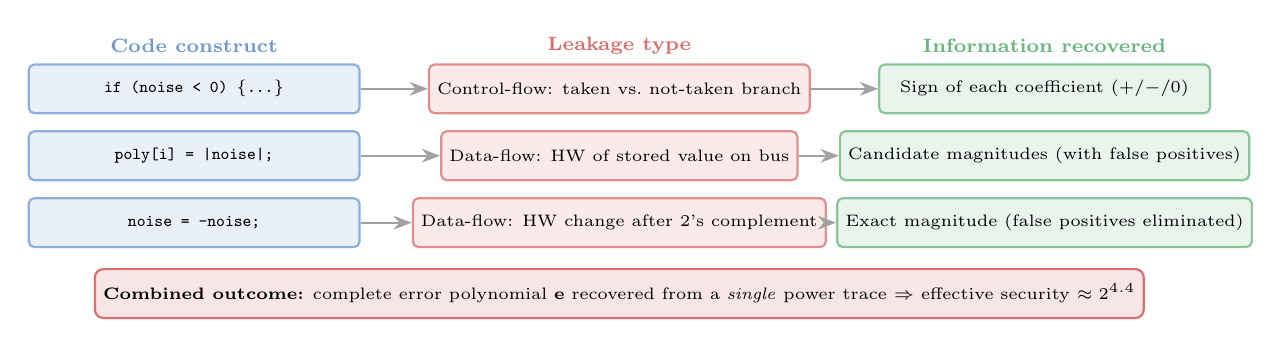
\begin{tikzpicture}[
  font=\fontsize{6.5pt}{8pt}\selectfont,
  >=Stealth,
  code/.style={rectangle, rounded corners=2pt, draw=cblu!55, thick,
               fill=cblu!10, minimum width=4.2cm, minimum height=0.62cm,
               text centered, inner sep=3pt,
               font=\fontsize{6.5pt}{8pt}\ttfamily},
  leak/.style={rectangle, rounded corners=2pt, draw=cred!55, thick,
               fill=cred!10, minimum width=4.2cm, minimum height=0.62cm,
               text centered, inner sep=3pt},
  sig/.style={rectangle, rounded corners=2pt, draw=cgrn!55, thick,
              fill=cgrn!10, minimum width=4.2cm, minimum height=0.62cm,
              text centered, inner sep=3pt},
  arr/.style={-{Stealth}, thick, cgry!60}
]
  %% Column headers
  \node[font=\fontsize{7pt}{9pt}\selectfont\bfseries, text=cblu!70]
    at (0,   0.55) {Code construct};
  \node[font=\fontsize{7pt}{9pt}\selectfont\bfseries, text=cred!70]
    at (5.4, 0.55) {Leakage type};
  \node[font=\fontsize{7pt}{9pt}\selectfont\bfseries, text=cgrn!70]
    at (10.8,0.55) {Information recovered};

  %% Row 1: branch
  \node[code] (c1) at (0,   0.00) {if (noise < 0) \{\ldots\}};
  \node[leak] (l1) at (5.4, 0.00) {Control-flow: taken vs.\ not-taken branch};
  \node[sig]  (s1) at (10.8,0.00) {Sign of each coefficient ($+$/$-$/0)};

  %% Row 2: store
  \node[code] (c2) at (0,  -0.85) {poly[i] = |noise|;};
  \node[leak] (l2) at (5.4,-0.85) {Data-flow: HW of stored value on bus};
  \node[sig]  (s2) at (10.8,-0.85) {Candidate magnitudes (with false positives)};

  %% Row 3: negation
  \node[code] (c3) at (0,  -1.70) {noise = -noise;};
  \node[leak] (l3) at (5.4,-1.70) {Data-flow: HW change after 2's complement};
  \node[sig]  (s3) at (10.8,-1.70) {Exact magnitude (false positives eliminated)};

  \draw[arr] (c1)--(l1); \draw[arr] (l1)--(s1);
  \draw[arr] (c2)--(l2); \draw[arr] (l2)--(s2);
  \draw[arr] (c3)--(l3); \draw[arr] (l3)--(s3);

  %% Outcome box
  \node[rectangle, rounded corners=3pt, draw=cred!70, fill=cred!12, thick,
        minimum width=13.2cm, minimum height=0.62cm, text centered, inner sep=3pt]
    at (5.4,-2.60) {\textbf{Combined outcome:} complete error polynomial $\mathbf{e}$
      recovered from a \emph{single} power trace $\Rightarrow$ effective security
      $\approx 2^{4.4}$};
\end{tikzpicture}
\caption{The three leakage channels of RevEAL, their corresponding code constructs,
  leakage type, and the information recovered at each stage. Combined, they yield
  the full error polynomial from a single power trace.}
\label{fig:leakage_channels}
\end{figure*}

\subsection{Step 5: Plaintext Recovery via LWE-with-Hints Lattice Attack}

Once the error polynomial $\mathbf{e}$ (or most of its coefficients) is known, the
attacker possesses far more information than a standard RLWE adversary. The
encryption equation
$c_0 = \mathbf{a}\cdot\mathbf{s} + \mathbf{e} + \Delta\mathbf{m}$
becomes, with $\mathbf{e}$ known:
\[
  c_0 - \mathbf{e} = \mathbf{a}\cdot\mathbf{s} + \Delta\mathbf{m}
\]
The adversary now seeks to recover $\mathbf{s}$ from $(\mathbf{a},\
c_0 - \mathbf{e})$, which is a standard RLWE instance \emph{without error}---or
more precisely, with an error that has been dramatically reduced because most of its
mass is now known.

The attacker frames this as an \emph{LWE-with-hints} problem and applies the
Distorted Bounded Distance Decoding (DBDD) framework of Espitau et al.~\cite{espitau2020},
which allows the known error coefficients to be incorporated as geometric hints
into the lattice problem. The resulting lattice has much lower dimension and shorter
shortest vector than the original RLWE lattice, making it solvable by
Block-Korkine-Zolotarev (BKZ) lattice reduction~\cite{bkz1994} at drastically
reduced cost. The quantitative impact is analysed in Section~\ref{sec:security}.

%%─────────────────────────────────────────────────────────────────────────────
\section{Quantitative Security Analysis}
\label{sec:security}
%%─────────────────────────────────────────────────────────────────────────────

\subsection{Security Metric: BKZ Block Size}

The standard metric for the hardness of an RLWE/LWE instance is the block size
$\beta$ required by BKZ to solve it. Larger $\beta$ corresponds to harder instances.
Following the approach of Espitau et al.~\cite{espitau2020}, Aydin et al.\ use the
relationship $\beta \cdot 2.98 \approx \log_2(\text{security bits})$ to convert BKZ
block sizes into equivalent bit
security~\cite{aydin2022reveal}. This conversion allows the impact of the side-channel
hints to be expressed in a meaningful security unit.

\subsection{Baseline Security}

For the SEAL-128 parameter set (designed for 128-bit post-quantum security), the
standard RLWE instance (without any side-channel leakage) requires a BKZ block size
of approximately $\beta = 382.25$. Converting: $382.25 \times 0.265 \approx 128$
bits (using the standard BKZ-to-security conversion), confirming the 128-bit
security claim. Equivalently, a brute-force attacker faces approximately $2^{128}$
work to recover the secret~\cite{aydin2022reveal}.

\subsection{Impact of Sign-Bit Leakage Alone}

The first leakage channel---the control-flow leak revealing the sign of each
coefficient---already has a catastrophic impact. When sign bits for all $n$
coefficients are provided as hints to the DBDD lattice framework, the required BKZ
block size drops from $\beta = 382.25$ to $\beta = 253.29$, a reduction of almost
130 blocks. Converting to bits: $253.29 \times 0.332 \approx 84.3$ bits of
security~\cite{aydin2022reveal}. This represents a reduction of more than $2^{43}$
in attack complexity---solely from knowing whether each noise sample was positive
or negative. The result is significant because the sign bits alone (without any
magnitude information) are recoverable with 100\% success from a single
trace~\cite{aydin2022reveal}.

\subsection{Impact of Full Leakage}

When all three leakage channels are exploited---sign bits from the branch, magnitudes
from the HW of stored values, and disambiguation from the negation---the attacker
recovers essentially the complete error polynomial. With these hints, the BKZ block
size required drops to $\beta \approx 12.2$. Converting: $12.2 \times 0.332
\approx 4.4$ bits of security---a \emph{complete break} of the scheme with
negligible computational cost~\cite{aydin2022reveal}.

Table~\ref{tab:security_impact} summarises these results.

\begin{table}[h]
\caption{Security Impact of RevEAL Leakage on SEAL-128 Parameter Set.}
\label{tab:security_impact}
\small
\begin{tabularx}{\columnwidth}{@{}X p{1.5cm} p{1.7cm}@{}}
\toprule
\textbf{Attack Scenario} & \textbf{BKZ Block Size $\beta$} & \textbf{Effective Security} \\
\midrule
No leakage (baseline) & 382.25 & $\approx 2^{128}$ \\
Sign-bit leak only (branch) & 253.29 & $\approx 2^{84.3}$ \\
Sign + magnitude (branch + store) & $\approx$200 & $\approx 2^{66}$ \\
Full leak (branch + store + negation) & 12.2 & $\approx 2^{4.4}$ \\
\bottomrule
\end{tabularx}
\end{table}

Figure~\ref{fig:security_reduction} visualises the progressive security degradation
across the three leakage channels.

\begin{figure}[h]
\centering
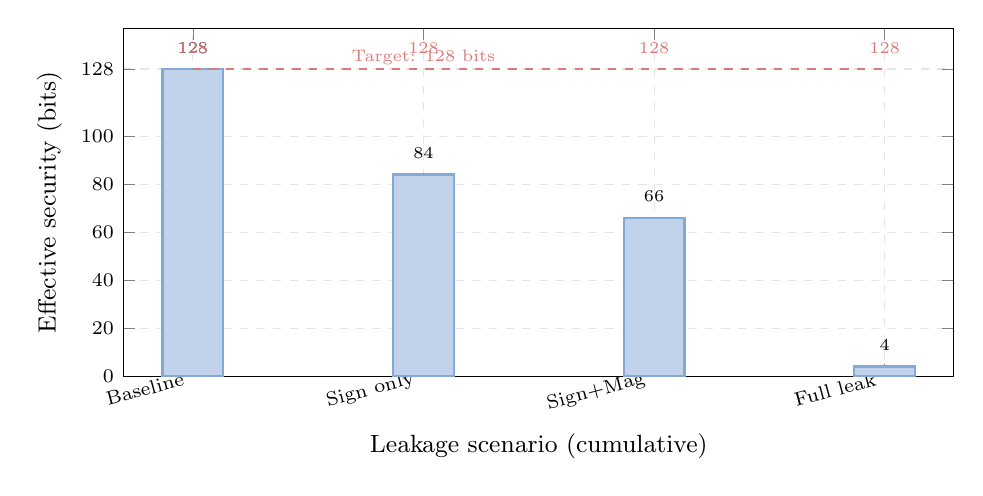
\begin{tikzpicture}
\begin{axis}[
  width=\columnwidth, height=6.0cm,
  xlabel={Leakage scenario (cumulative)},
  ylabel={Effective security (bits)},
  xlabel style={font=\small},
  ylabel style={font=\small},
  symbolic x coords={Baseline, Sign only, Sign+Mag, Full leak},
  xtick=data,
  x tick label style={font=\scriptsize, rotate=15, anchor=east},
  ymin=0, ymax=145,
  ytick={0,20,40,60,80,100,128},
  yticklabel style={font=\scriptsize},
  grid=major, grid style={dashed, gray!20},
  bar width=22pt,
  nodes near coords,
  nodes near coords align={vertical},
  nodes near coords style={font=\fontsize{6.5pt}{8pt}\selectfont, yshift=2pt}
]
  \addplot[
    ybar,
    fill=cblu!30, draw=cblu!60, thick
  ] coordinates {
    (Baseline, 128)
    (Sign only, 84)
    (Sign+Mag, 66)
    (Full leak, 4)
  };
  \addplot[
    mark=none, dashed, thick, cred!65
  ] coordinates {
    (Baseline, 128) (Sign only, 128) (Sign+Mag, 128) (Full leak, 128)
  };
  \node[font=\fontsize{6pt}{7.5pt}\selectfont, text=cred!65]
    at (axis cs:Sign only, 133) {Target: 128 bits};
\end{axis}
\end{tikzpicture}
\caption{Progressive security degradation under RevEAL leakage. The dashed red line
  marks the 128-bit security target. Full exploitation of all three leakage channels
  reduces security to approximately $2^{4.4}$ bits---effectively zero.}
\label{fig:security_reduction}
\end{figure}

\subsection{Interpretation}

These numbers reveal a structural danger in applying mathematical security arguments
to physically implemented cryptography. The BFV scheme, as a mathematical object, is
128-bit secure for the SEAL-128 parameter set; no known algorithm breaks it within
that bound. Yet a physical measurement of the device during \emph{one} encryption
reduces this to $2^{4.4}$---not because the mathematics is wrong, but because the
implementation discloses secret data through its physical behaviour. The proof of
security makes no claim about implementation; RevEAL exposes the gap.

%%─────────────────────────────────────────────────────────────────────────────
\section{Why Masking Fails: Single-Trace Structural Argument}
\label{sec:masking}
%%─────────────────────────────────────────────────────────────────────────────

\subsection{The Standard Masking Defence}

Masking is the dominant hardware countermeasure against power analysis. In its basic
form, a secret value $v$ is split into $d+1$ shares $(v_0, v_1, \ldots, v_d)$ such
that $v = v_0 \oplus v_1 \oplus \cdots \oplus v_d$, where each share is
independently and uniformly random. Every operation on $v$ is performed share-by-share,
so the power consumption at each step depends on a random mask rather than on $v$
itself. An attacker who observes power traces for many executions cannot recover $v$
because each trace involves different random masks---the leakage is decorrelated from
the secret.

Masking provides provably secure protection at order $d$ against $d$th-order DPA:
an attacker who observes the joint distribution of $d$ trace points cannot recover
the secret, even with infinitely many traces, as long as the shares are
uniformly random~\cite{ishai2003}.

\subsection{Why Masking Does Not Apply to RevEAL}

The fundamental assumption of masking's security proof is that the attacker combines
information from \emph{multiple executions} (with different masks each time) to
cancel the masking noise. RevEAL violates this assumption at a structural level:

\begin{enumerate}
\sloppy
  \item \textbf{Fresh randomness per encryption.} In SEAL's BFV encryption, the
        noise polynomial $\mathbf{e}$ is drawn fresh for every encryption. There is
        no fixed secret value being encrypted repeatedly; the noise itself is
        the target, and it changes every time. There are therefore no ``many traces
        of the same secret'' to combine. As Aydin et al.\ note: ``multi-trace attacks
        \ldots do not work by default on the encryption'' process~\cite{aydin2022reveal}.

  \item \textbf{Single-trace sufficiency.} RevEAL recovers the sign of each coefficient
        with 100\% accuracy from \emph{one} trace~\cite{aydin2022reveal}. The branch
        leakage is not a statistical signal that requires averaging to surface---it
        is a direct, deterministic instruction-count difference between the taken and
        not-taken paths. Masking does not eliminate this: a masked computation would
        still branch on the unmasked (or remasked) sign bit at some point in the
        computation, recreating the leakage.

  \item \textbf{Template attack optimality.} The template-matching approach used in
        Step~2 of RevEAL is information-theoretically optimal for single-trace
        analysis~\cite{chari2002}. Masking adds noise to individual measurements,
        but with a single observation the attacker uses the template to make the best
        possible inference from the available signal. Unless masking eliminates the
        distinguishing signal \emph{entirely} (which requires that the masked and
        unmasked paths produce identically distributed power traces---an extremely
        strong requirement), template matching will still succeed with some
        probability.
\end{enumerate}

The paper states this conclusion directly: ``Since we apply a single-trace
side-channel analysis, masking \ldots [is] not effective''~\cite{aydin2022reveal}.
The authors do not merely assert this; it follows from the structure of the
attack. Figure~\ref{fig:masking_analysis} formalises why masking addresses a
different threat model than RevEAL.

\begin{figure}[h]
\centering
\scalebox{0.87}{
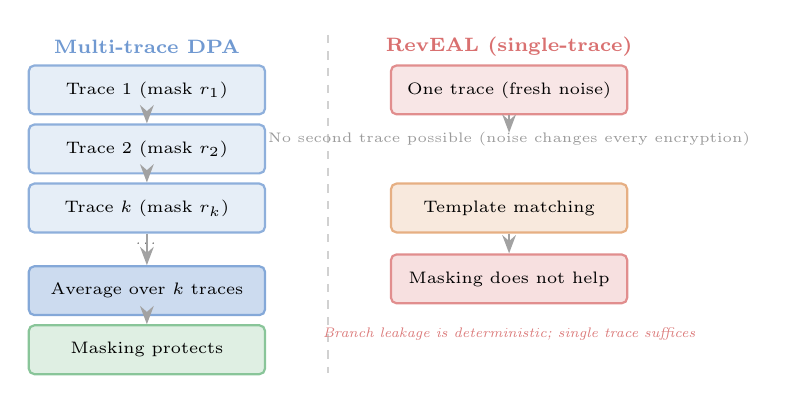
\begin{tikzpicture}[
  font=\fontsize{6.5pt}{8pt}\selectfont,
  >=Stealth,
  box/.style={rectangle, rounded corners=2pt, draw, thick,
              minimum width=3.0cm, minimum height=0.62cm,
              text centered, inner sep=3pt},
  arr/.style={-{Stealth}, thick, cgry!60}
]
  %% Left: DPA / masking threat model
  \node[font=\fontsize{7pt}{9pt}\selectfont\bfseries, text=cblu!70]
    at (-2.3, 0.55) {Multi-trace DPA};
  \node[box, fill=cblu!12, draw=cblu!55] (dt1) at (-2.3, 0.00) {Trace 1 (mask $r_1$)};
  \node[box, fill=cblu!12, draw=cblu!55] (dt2) at (-2.3,-0.75) {Trace 2 (mask $r_2$)};
  \node[box, fill=cblu!12, draw=cblu!55] (dt3) at (-2.3,-1.50) {Trace $k$ (mask $r_k$)};
  \node[font=\fontsize{5.5pt}{7pt}\selectfont\itshape, text=cgry]
    at (-2.3,-1.95) {\ldots};
  \node[box, fill=cblu!25, draw=cblu!60] (av) at (-2.3,-2.55) {Average over $k$ traces};
  \node[box, fill=cgrn!15, draw=cgrn!55] (sec) at (-2.3,-3.30) {Masking protects};
  \draw[arr] (dt1)--(dt2); \draw[arr] (dt2)--(dt3);
  \draw[arr] (dt3)--(av); \draw[arr] (av)--(sec);

  %% Divider
  \draw[dashed, cgry!30] (0, 0.70) -- (0,-3.60);

  %% Right: RevEAL single-trace model
  \node[font=\fontsize{7pt}{9pt}\selectfont\bfseries, text=cred!70]
    at ( 2.3, 0.55) {RevEAL (single-trace)};
  \node[box, fill=cred!12, draw=cred!55] (st1) at ( 2.3, 0.00) {One trace (fresh noise)};
  \node[font=\fontsize{5.5pt}{7pt}\selectfont, text=cgry!65, align=center]
    at ( 2.3,-0.62) {No second trace possible (noise changes every encryption)};
  \node[box, fill=cora!15, draw=cora!55] (tm) at ( 2.3,-1.50) {Template matching};
  \node[box, fill=cred!15, draw=cred!55] (fail) at ( 2.3,-2.40) {Masking does not help};
  \node[font=\fontsize{5.5pt}{7pt}\selectfont\itshape, text=cred!65, align=center]
    at ( 2.3,-3.10) {Branch leakage is deterministic; single trace suffices};
  \draw[arr] (st1.south) -- ++(0,-0.22);
  \draw[arr] (tm)--(fail);
\end{tikzpicture}
}%
\caption{Structural comparison between the multi-trace DPA threat model (for which
  masking is designed) and the single-trace RevEAL threat model (for which masking
  provides no protection). Masking addresses statistical averaging across many
  traces; RevEAL requires only one.}
\label{fig:masking_analysis}
\end{figure}

%%─────────────────────────────────────────────────────────────────────────────
\section{Recommended Defenses and Trade-offs}
\label{sec:defenses}
%%─────────────────────────────────────────────────────────────────────────────

\subsection{Constant-Time Sampling: Eliminating Secret-Dependent Branches}

The root cause of the RevEAL vulnerability is that the implementation branches on
the sign of a secret value. The principled fix is to eliminate this branch entirely
by rewriting the sampling code in constant time: every iteration of the loop executes
the same sequence of instructions regardless of the sampled value.

There are several concrete approaches. First, the code can use
\emph{arithmetic select operations} (a.k.a.\ conditional moves or masking): compute
both the positive and negative representations, then select the correct one using a
non-branching mask derived from the sign bit:

\begin{lstlisting}[label=lst:fixed, caption={Constant-time sign handling without branching.}]
int64_t mask = noise >> 63; // all-1s if negative, 0 otherwise
int64_t abs_val = (noise ^ mask) - mask; // |noise|, no branch
poly[i] = abs_val;          // same instruction always
// restore sign arithmetically if needed
\end{lstlisting}

This code performs exactly the same operations whether \texttt{noise} is positive or
negative. There is no branch and no instruction-count difference, so control-flow
leakage is eliminated.

Second, and more fundamentally, SEAL v3.6 replaced Gaussian sampling with
\emph{centered binomial distribution} (CBD) sampling as the default~\cite{sealchanges}.
CBD generates noise by computing $b = \sum_{i=1}^{k} a_i - \sum_{i=1}^{k} a_i'$
where each $a_i, a_i' \in \{0,1\}$ is a uniformly random bit. This can be implemented
entirely with XOR, AND, and population-count operations---no branching on any secret
value is required~\cite{sealchanges}. The Microsoft changelog explicitly notes: ``sampling
from a CBD is constant-time \ldots which is why it is used by many of the NIST PQC
finalists''~\cite{sealchanges}. CBD is also faster than Gaussian sampling on modern
hardware, because it avoids rejection sampling.

\textbf{Trade-off.} CBD does not produce a true Gaussian distribution; it approximates
one with binomial tails. For most practical parameter sets the approximation is
mathematically acceptable (the noise distribution must merely be bounded and small),
but for applications requiring certified Gaussian noise (rare in practice) a
constant-time Gaussian sampler using the algorithm of Ducas et al.\ or the table-based
CDT method must be used.

\subsection{Shuffling and Index Randomisation}

Even after eliminating the branch vulnerability, the data-flow leakage (HW of stored
values) remains a potential threat. A complementary defence is to process coefficients
in a randomised order: instead of iterating from $i=0$ to $i=n-1$, the code uses a
random permutation of indices. This disconnects the mapping between trace position
and polynomial index, forcing the attacker to guess the permutation before the
template can be matched~\cite{aydin2022reveal}.

The RevEAL authors specifically recommend ``shuffling or other forms of
randomization/obfuscation''~\cite{aydin2022reveal}. Shuffling adds $O(n)$ overhead
(generating a random permutation of $n$ elements) and introduces some additional
branches for the permutation generation---which must themselves be constant-time.
If the branch vulnerability is already eliminated through constant-time coding,
shuffling provides defense-in-depth against the magnitude leakage channel.

\subsection{Residual Risks and Implementation Vigilance}

Aydin et al.\ caution that version~3.6 and later ``may have a different
vulnerability''~\cite{aydin2022reveal}---the fixing of one leakage channel does not
guarantee the absence of others. This is a general principle of implementation
security: any operation that processes secret data can potentially leak information
through some physical channel. Constant-time coding eliminates the known leakage
channels, but library developers must maintain ongoing vigilance through:

\begin{itemize}
  \item Code review and static analysis for data-dependent branches in any
        cryptographic routine
  \item Formal verification tools (e.g., ct-verif, binsec) that certify
        constant-time execution
  \item Periodic re-evaluation of the noise sampling code as the SEAL codebase
        evolves
  \item Physical leakage testing (TVLA: Test Vector Leakage Assessment~\cite{goodwill2011})
        on representative hardware
\end{itemize}

Table~\ref{tab:defenses} provides a structured comparison of the recommended defenses.

\begin{table*}[t]
\caption{Summary of RevEAL Leakage Points, Attack Techniques, and Countermeasures.}
\label{tab:defenses}
\small
\begin{tabularx}{\textwidth}{@{}p{2.4cm}p{1.8cm}Xp{3.5cm}p{1.5cm}@{}}
\toprule
\textbf{Leakage Point} & \textbf{Leakage Type} & \textbf{Attack Technique} & \textbf{Countermeasure} & \textbf{Overhead} \\
\midrule
\texttt{if (noise < 0)} & Control-flow & Template match on branch outcome; recovers sign bit with 100\% accuracy & Constant-time code: arithmetic masking, or switch to CBD sampling & Negligible \\
\addlinespace[3pt]
\texttt{poly[i] = |noise|} & Data-flow (HW) & HW template matching on stored value; recovers magnitude candidates & Shuffled coefficient order; constant-time store & $O(n)$ permutation \\
\addlinespace[3pt]
\texttt{noise = -noise} & Data-flow (HW shift) & HW change after 2's complement resolves false positives & Eliminate explicit negation; use arithmetic sign selection & Negligible \\
\addlinespace[3pt]
Combined all three & Both & BKZ/DBDD with full hints; $\beta = 12.2$ ($\approx 2^{4.4}$) & All of the above; use SEAL v3.6+ with CBD default & Minimal \\
\bottomrule
\end{tabularx}
\end{table*}

%%─────────────────────────────────────────────────────────────────────────────
\section{Discussion}
%%─────────────────────────────────────────────────────────────────────────────

\subsection{The Implementation-Security Gap in FHE}

The RevEAL attack illustrates a structural gap that is particularly acute for
homomorphic encryption. HE schemes are designed to prove their security through
reductions to hard lattice problems, and the mathematical argument is rigorous.
However, the proof model treats the encryption oracle as a black box that receives
no side-channel signal; the physical implementation is not part of the security
model. This gap is not unique to HE---the same issue affects RSA, elliptic curve,
and AES implementations---but it is more dangerous in the HE context for two reasons.

First, HE is increasingly being deployed in high-value settings: privacy-preserving
machine learning inference, secure database queries, and medical record computation.
The data being processed is often highly sensitive. A single power measurement of
the device during an encryption operation is all that is required to break the
scheme completely.

Second, the FHE community has historically focused its security analysis on the
hardness of the underlying mathematical problem, with less attention to implementation
security. The RevEAL paper serves as a corrective: it demonstrates that an adversary
who bypasses the mathematical hardness through physical observation can achieve
complete decryption with an attack cost of $2^{4.4}$.

\subsection{Generalisability of the Attack}

The RevEAL methodology is not specific to SEAL or to the BFV scheme. Any HE library
that samples error polynomials using code with secret-dependent branches or
data-dependent memory writes is potentially vulnerable to the same approach. The
CKKS scheme (also implemented in SEAL) uses a similar Gaussian sampling routine and
would be subject to analogous analysis. Implementations of the BGV scheme and of
TFHE that use discrete Gaussian sampling may have similar exposure.

The attack methodology generalises to any lattice-based cryptographic scheme that
relies on a noise sampling subroutine: lattice-based key encapsulation mechanisms
(ML-KEM, formerly CRYSTALS-Kyber) and digital signatures (ML-DSA, formerly
CRYSTALS-Dilithium) also sample small polynomials during key generation or signing.
NIST's standardised PQC algorithms address this explicitly: ML-KEM uses centered
binomial sampling (the same fix that SEAL v3.6 adopted) precisely because it is
implementable in constant time without branches on secret data.

\subsection{Lesson for Practitioners}

The practical lesson from RevEAL is unambiguous: cryptographic security proofs do not
protect against implementation vulnerabilities. Practitioners deploying HE in
production environments must:

\begin{enumerate}
  \item Use current, patched library versions (SEAL v3.6+ with CBD default, or any
        equivalent constant-time FHE implementation).
  \item Treat all code that processes secret data---including noise sampling, key
        generation, and decryption---as a potential leakage source, and apply
        constant-time principles throughout.
  \item Understand that masking, random delays, and hardware shielding are not
        substitutes for correct algorithm implementation. They may raise the bar for
        exploitation on certain hardware platforms, but they do not eliminate
        single-trace leakage arising from deterministic branch differences.
  \item Perform physical leakage testing (TVLA) on the target hardware before
        production deployment.
\end{enumerate}

%%─────────────────────────────────────────────────────────────────────────────
\section{Conclusion}
%%─────────────────────────────────────────────────────────────────────────────

The RevEAL attack demonstrates that mathematical security of a homomorphic encryption
scheme provides no guarantee against an adversary who can measure the physical device
executing the encryption. By exploiting three specific implementation choices in
SEAL's Gaussian sampling routine---a conditional branch on the sign of each
coefficient, a data-dependent memory write of the absolute value, and a 2's-complement
negation---an attacker can recover the complete error polynomial from a single power
trace, reducing a 128-bit-secure scheme to effective security of approximately
$2^{4.4}$ bits. Sign-bit leakage alone is sufficient to reduce security to
$2^{84.3}$ with 100\% accuracy using template analysis.

Conventional masking defenses are structurally ineffective against RevEAL because
they address the multi-trace threat model, while RevEAL requires only a single
measurement. The fresh randomness used in each encryption prevents multi-trace
accumulation, and the branch leakage is deterministic---not statistical---so
averaging provides no benefit to the defender.

The correct defense is at the code level: replacing secret-dependent branches with
constant-time arithmetic operations, and switching to centered binomial distribution
sampling, which requires no branching on secret values. Microsoft adopted both
measures in SEAL v3.6, and the NIST PQC standardisation process mandated CBD sampling
for ML-KEM for precisely the same reason. The broader lesson is that implementation
security must be treated as a first-class requirement in any cryptographic library,
not as an afterthought to the mathematical design. RevEAL makes clear that for FHE,
as for all practical cryptography, a scheme is only as secure as the code that runs it.

\begin{acks}
The author acknowledges the foundational contributions of Aydin et al.\ whose RevEAL
paper provided the empirical basis for this analysis, and the broader lattice
cryptography and side-channel communities whose prior work in template attacks and
LWE-with-hints made the attack framework possible.
\end{acks}

\sloppy
\bibliographystyle{ACM-Reference-Format}
\begin{thebibliography}{25}

\bibitem{aydin2022reveal}
A.~Aydin, A.~Abdulrahman, K.~Yuce, T.~Scholl, P.~Sasdrich, and T.~Schneider. 2022.
RevEAL: Single-Trace Side-Channel Leakage of the SEAL Homomorphic Encryption Library.
\textit{IACR ePrint} 2022.

\bibitem{brakerski2012}
Z.~Brakerski, C.~Gentry, and V.~Vaikuntanathan. 2012. (Leveled) Fully Homomorphic
Encryption without Bootstrapping. In \textit{Proc.\ ITCS 2012}. ACM, 309--325.

\bibitem{fan2012}
J.~Fan and F.~Vercauteren. 2012. Somewhat Practical Fully Homomorphic Encryption.
\textit{IACR ePrint} 2012/144.

\bibitem{sealcrypto}
Microsoft Research. 2022. \textit{Microsoft SEAL (Simple Encrypted Arithmetic Library)}.
Version 3.7. \url{https://github.com/microsoft/SEAL}

\bibitem{sealchanges}
Microsoft Research. 2021. SEAL CHANGES.md: Version 3.6 Release Notes.
\url{https://github.com/microsoft/SEAL/blob/main/CHANGES.md}

\bibitem{kocher1999}
P.~Kocher, J.~Jaffe, and B.~Jun. 1999. Differential Power Analysis. In
\textit{Advances in Cryptology---CRYPTO 1999}, LNCS vol.~1666. Springer, 388--397.

\bibitem{messerges2000}
T.~S.~Messerges, E.~A.~Dabbish, and R.~H.~Sloan. 2000. Examining Smart-Card Security
under the Threat of Power Analysis Attacks. \textit{IEEE Trans.\ Comput.} 51, 5
(2002), 541--552.

\bibitem{chari2002}
S.~Chari, J.~R.~Rao, and P.~Rohatgi. 2002. Template Attacks. In
\textit{Cryptographic Hardware and Embedded Systems---CHES 2002}, LNCS vol.~2523.
Springer, 13--28.

\bibitem{walter2001}
C.~D.~Walter. 2001. Sliding Windows Succumbs to Big Mac Attack. In
\textit{CHES 2001}, LNCS vol.~2162. Springer, 286--299.

\bibitem{mangard2007}
S.~Mangard, E.~Oswald, and T.~Popp. 2007. \textit{Power Analysis Attacks: Revealing
the Secrets of Smart Cards}. Springer.

\bibitem{espitau2020}
T.~Espitau, A.~Joux, and N.~Kharchenko. 2020. On a Hybrid Approach to Solve Small
Secret LWE. In \textit{ASIACRYPT 2020}, LNCS vol.~12492. Springer, 515--544.

\bibitem{bkz1994}
C.~P.~Schnorr and M.~Euchner. 1994. Lattice Basis Reduction: Improved Practical
Algorithms and Solving Subset Sum Problems. \textit{Mathematical Programming}
66 (1994), 181--191.

\bibitem{ravi2019}
P.~Ravi, S.~Bhasin, S.~S.~Roy, and A.~Chattopadhyay. 2019. Side-Channel Assisted
Existential Forgery Attack on Dilithium. \textit{IACR ePrint} 2018/821.

\bibitem{pessl2019}
P.~Pessl, L.~Bruinderink, and Y.~Yarom. 2019. To BLISS-B or not to be: Attacking
strongSwan's Implementation of Post-Quantum Signatures. In
\textit{Proc.\ ACM CCS 2017}. ACM, 1843--1855.

\bibitem{ishai2003}
Y.~Ishai, A.~Sahai, and D.~Wagner. 2003. Private Circuits: Securing Hardware against
Probing Attacks. In \textit{CRYPTO 2003}, LNCS vol.~2729. Springer, 463--481.

\bibitem{goodwill2011}
G.~Goodwill, B.~Jun, J.~Jaffe, and P.~Rohatgi. 2011. A Testing Methodology for
Side-Channel Resistance Validation. NIST Non-Invasive Attack Testing Workshop.

\bibitem{rfc2401}
NIST. 2024. \textit{FIPS 203: Module-Lattice-Based Key-Encapsulation Mechanism
Standard (ML-KEM)}. National Institute of Standards and Technology.

\end{thebibliography}

\end{document}
